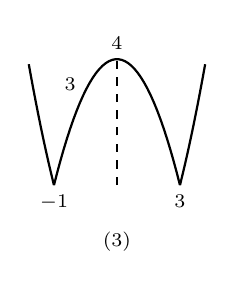
\begin{tikzpicture}[scale=0.4]
\ax{-2}{4.2}{-0.8}{5}
\draw[thick,domain=-1.8:-1,samples=20] plot (\x,{(\x-1)^2-4});
\draw[thick,domain=-1:3,samples=40] plot (\x,{4-(\x-1)^2});
\draw[thick,domain=3:3.8,samples=20] plot (\x,{(\x-1)^2-4});
\draw[dashed] (1,0)--(1,4);
\node[below] at (-1,0){\scriptsize $-1$}; \node[below] at (3,0){\scriptsize 3};
\node[above] at (1,4){\scriptsize 4}; \node[left] at (0,3.2){\scriptsize 3};
\node at (1,-1.8){\scriptsize (3)};
\end{tikzpicture}